
%----------------------------------------------------------------------------------------
%	3./ Observing mode
%----------------------------------------------------------------------------------------
%\section{Observations}
%\label{se:observations}

This section presents the different observation modes that are used at
the \trentemetre\ IRAM telescope for both commissioning and
scientific-purpose observations with NIKA2. {\lp Each observation
campaign is organized as observing pool allowing to optimize
observations of several science targets in a flexible way.}
Most of the used observing scans are based on on-the-fly raster scans,
which consists of several linear scanning legs, combined to one
map. Their characteristics have been tailored for NIKA2 performance.
%Some of them are common
%to usual IRAM observing modes (\emph{e.g.}~''on the fly'' raster scans), some of them
%have been designed specifically for \nika\ (e.g.~the focus sequence).
% \todo{define PAKO}

%\subsection{Overview of different types of scans}

%Once the KIDs are tuned and \nika\ is ready for observations, before actually
%observing a scientific target, one needs to adjust the focus and pointing of the
%telescope. In the case of EMIR typically, these two parameters are adjusted iteratively by
%alterning ``pointing'' (\aka\ ``cross'') and ``focus'' scans to optimize the
%centering of a bright point source on a reference detector and to maximize the
%incoming flux on it. With \nika\ , mostly due to absence of horns, this
%procedure is not optimal. Indeed, it was noticed that the position of the source
%moved by several arcsec with the displacement of M2
%during the focus procedure and this would alter the flux
%measurement on a fixed reference position too much to enable focus
%optimization.

%\begin{figure*}[!thbp]
%\begin{center}
%  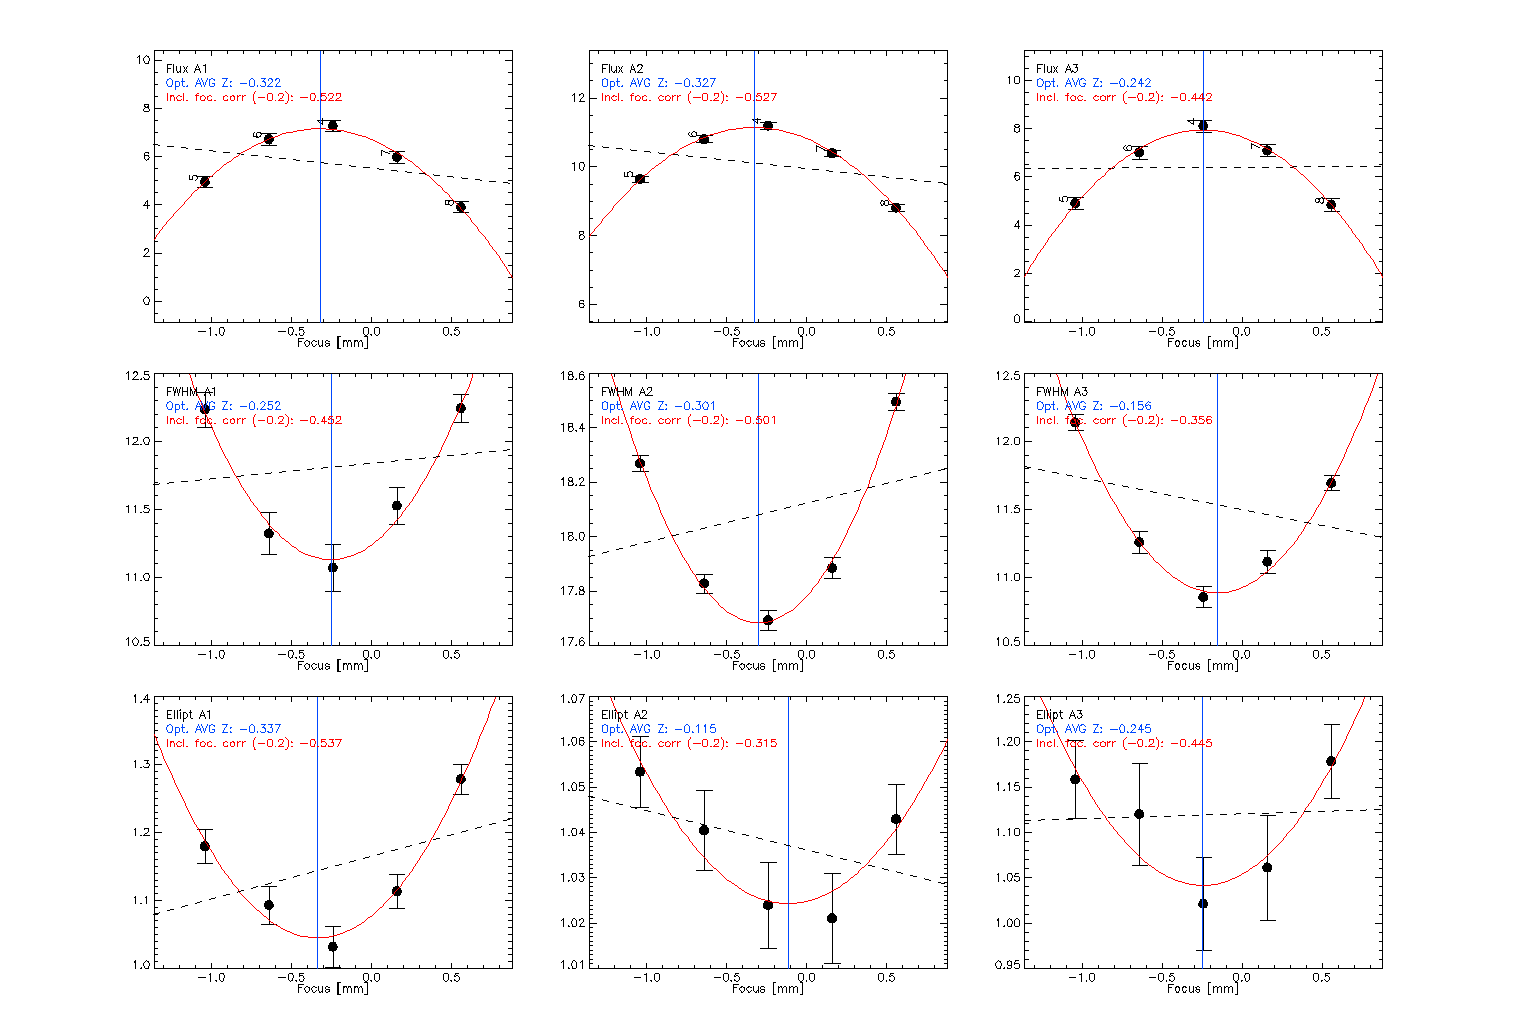
\includegraphics[clip, angle=0, trim={3cm, 12cm, 3cm, 1.5cm}, width=0.75\textwidth]{Figures/plot_20180120s8_zfocus.png}
%\caption[]{Example of axial focus measurement using a dedicated focus
%  observation sequence of the bright quasar 3C84 during the Juanuary
%  2018 campaign (N2R14) in good observing conditions. Flux (first
%  row) and FWHM (second row) measurements are
%  shown as a function of the axial focus offsets for Array 1 (first
%  column), Array 2 (second column) and Array 3 (third column). The
%  best-fitting parabola is shown in red. To help the observer
%  assessing the parabolic fit quality, the best-fit linear model is also drawn
%  with dashed black lines. 
%  The blue vertical line locates the best-fitting $z$-focus value of
%  each fit. The optimal focus values derived from flux
%  maximization and FWHM minimization agree to better than 0.1\,mm in these
%  conditions of observation. %While ellipticity may be often regarded as a confirmation
%  %more than a decisive criterion (due to larger uncertainty on its measure), the
%  %associated minimum is also in good agreement with the values derived from flux
%  %and FWHM measurements in this example taken in stable atmospheric
%  %conditions.
%}
%\label{fig:focus-example}
%\end{center}
%\end{figure*}

\subsection{Focus}
\label{se:axial_focus}

Observation pools start with setting the telescope focus since NIKA2 large
FOV alleviates the need to adjust the pointing beforehand.  
We have designed a specific focus procedure that takes
advantage of the dense sampling of the FOV allowing to map a source
in a short integration time. We perform a series of five successive one-minute
raster scans of a bright (above a few Jy) point source at five
axial offsets of the secondary mirror (M2) along the optical
axis. As the scan size is $1'\times 5'$, the main contribution to each
map mainly comes from the KIDs located in the central part of the FOV.%, typically
%$\{-0.8, -0.4, 0, 0.4, 0.8\}$\,mm w.r.t.~the current $z$-focus (which
%is usually the previous optimal $z$-focus value).
%We then analyse each map to optimize the $z$ position of M2.

%More details are given in
%Sect.~\ref{se:axial_focus}.
%Once the focus is correctly determined, the pointing
%corrections are derived from an EMIR like pointing calibration scan
%(Sect.~\ref{se:pointing}). The instrument is then ready to observe scientific
%targets.

%\subsection{Axial focus}
%\label{se:axial_focus}

%The best axial focus in the central region of the arrays is estimated
%using the
%so-called {\tt focus$\_$OTF} PAKO script, which produces a series of
%five $1'\times 5'$ OTF scans at various values of the focus in $0.4~\rm{mm}$ steps
%around an \emph{a priori} value $z_0$, namely
%$z \in \{-0.8, -0.4, 0, 0.4, 0.8\} + z_0$.
Elliptical Gaussian fits on the five maps provide estimates of
the flux and FWHM along minor and major axes for each focus. 
The best axial focus in the central part of the array is then
estimated as the maximum of the flux or the minimum of the FWHM using
parabolic fits of the five measurements.
%Parabolic fits are
%then used to determine the best focus.%, as illustrated in Fig.~\ref{fig:focus-example}.
%We consider three estimates: i) $\hat
%z_{\rm{peak}}$ the focus that maximizes the estimated flux, which is the
%amplitude of the 2D Gaussian, ii) $\hat z_{\rm{fwhm}}$ the focus that minimizes
%the geometrical FWHM, defined as the quadratic mean of $\rm{FWHM}_{\rm{major}}$
%and $\rm{FWHM}_{\rm{minor}}$, and iii) $\hat z_{\rm{ellipt}}$ the focus that
%minimizes the beam ellipticity, defined as
%$\rm{FWHM}_{\rm{major}}/\rm{FWHM}_{\rm{minor}}$. Fig.~\ref{fig:focus-example}
%shows an example of such a sequence. When deciding on the focus to apply, we
%give priority to the optimal flux, taking an average between values on A1 and
%A3: there is little difference between the two and the 2\,mm channel is
%less sensitive to the focus change than the 1\,mm.

As presented in more details in Appendix~\ref{ap:focus_surfaces}, the focus
surface, that is defined as the locations of the best focus across the whole FOV
is not strictly flat but rather bowl-shaped.
%The way sources are scanned in
%this {\tt focus\_OTF} sequence is designed to save time but it gives more weight
%to the central KIDs.
%Hence, the optimal focus derived from the fits is biased.
To account for the curvature of the focus surfaces and optimize the
average focus across the FOV, we add -0.2\,mm to the best axial focus
in the central part of the array. This focus offset is measured on data using
a dedicated sequence of de-focused scans, as discussed in
Appendix~\ref{ap:focus_surfaces}. It is in agreement with expectations
derived with optical simulation using ZEMAX\footnote{Web site: \tt{www.zemax.com}}. 

{\lp Axial focus offsets are measured every other hours during daytime and
are systematically checked after sunrises and sunsets, while one or
two checks suffice during night. 
Lateral focus offsets can also be checked in a similar way, but are
found to stay constant over periods of time that cover several
observing campaigns.}


%\subsection{Lateral focus}
%\label{sec:focus_X_Y}

%Like in the $z$ (optical axis) direction, it is possible to control the position
%of M2 along the $x$ and $y$ directions. We have tried to determine if there was
%an optimal position in the $(x,y)$ plane that would improve further measurements
%with \nika. We have applied the same procedure as the one described in
%Sect~\ref{se:axial_focus}, this time varying the position of M2 along $x$ or $y$
%rather than along $z$. Examples of such observations are presented on
%Figs.~\ref{fig:X_focus} and \ref{fig:Y_focus}. While the forced parabola fit
%guides the eye towards optimization, one should note the size of the error bars
%and the relatively low variations compared to M2 displacements along the $z$
%axis. This is expected from optical simulations and experience on
%EMIR. Figs.~\ref{fig:X_focus} and \ref{fig:Y_focus} also show as complement,
%images of the residuals of the intensity maps at each M2 position after the
%subtraction of an elliptical gaussian fitted only on a disk of 6 and 15\,arcsec
%(1 and 2\,mm resp.) around the maximum location and outside a ring of 100\,arcsec
%away from the maximum (to fix the background while not being affected by the
%side lobes). These maps of residuals are meant to help to decide on a minimization
%criterion and $x$ or $y$-focus value.

%While we have performed ``many'' of such observations and explored the entire
%parameter space of the $(x,y,z)$~triplet position in a reasonable range of
%several millimeters around a fixed position, it has not been possible to
%demonstrate that any $(x,y)$ positions would improve significantly the
%focusing of the whole system compared to the nominal $(0,0)$ reference
%position. \vu{This confirms the experience of the IRAM staff with EMIR and
%HERA who only act on this $(x,y)$ position about once a year after
%specific, dedicated and delicate measures. This effort is necessary
%to find an optimum lateral focus position which is stable with
%elevation. For \nika\, the adopted strategy has been not to change the
%lateral focus parameters and only rely on $z$-focus optimization for
%observations. However, lateral focus measurements with NIKA2 have to be
%scheduled in the future.} 

%\begin{figure*}[h!]
%\centering
%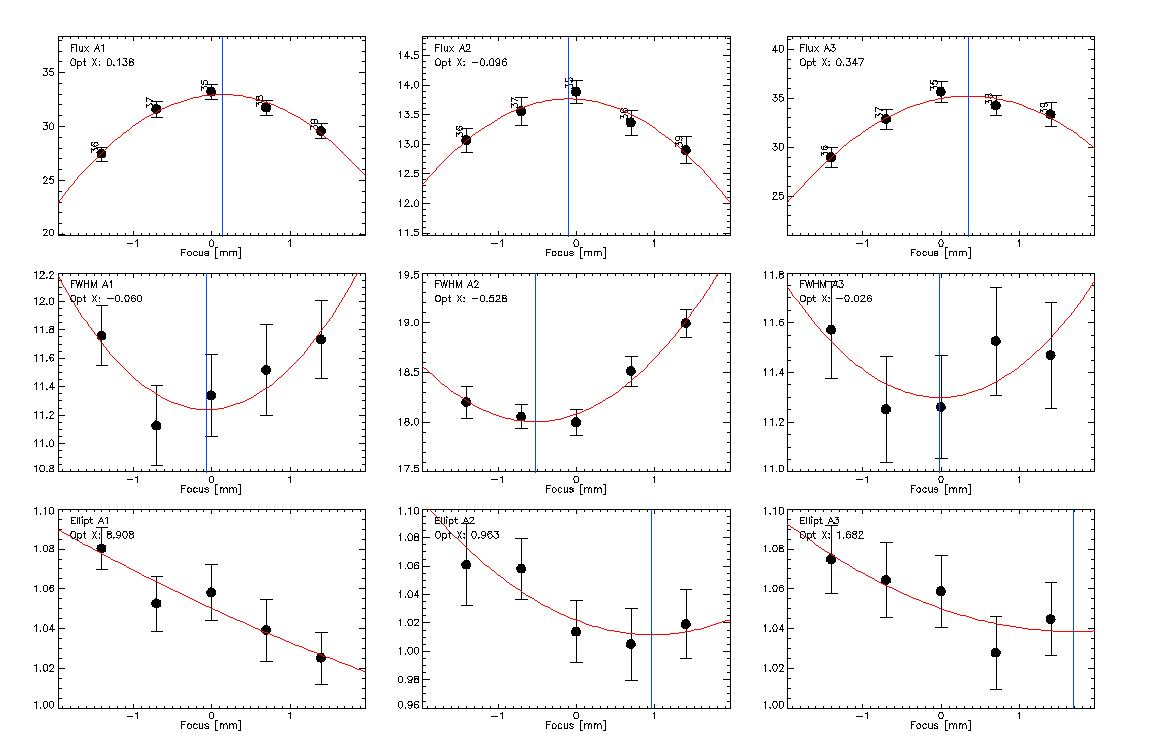
\includegraphics[height=8cm]{Figures/plot_20170223s39.png}
%\hspace{0.5cm}
%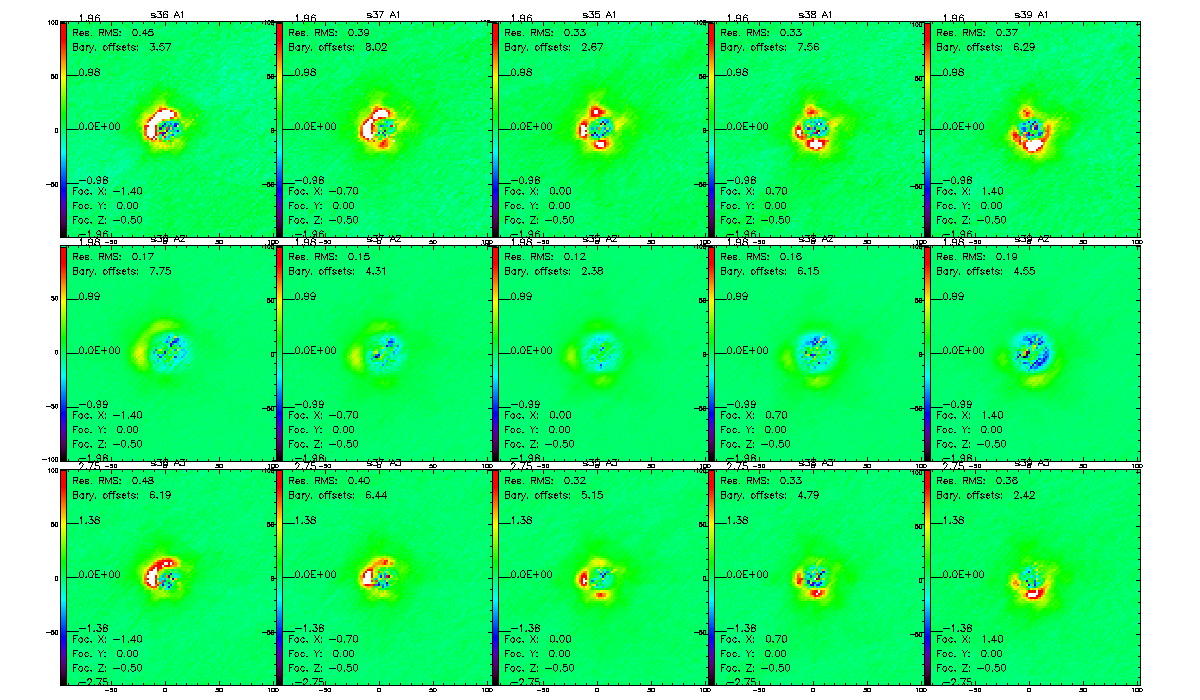
\includegraphics[height=8cm]{Figures/residuals_focus_otf_20170223s39.png}
%\caption[Lateral X focus measurements]{\emph{top panel: }X-focus measurement using a
%    parabolic fit of the flux, beam FWHM and ellipticity on a sequence
%    of five OTF scans on Uranus (20170223s39-43) \emph{bottom panel: }Beam residuals
%    after subtracting a model of the main beam for each OTF-scan of the X-focus
%    session. (N2R9)}
%\label{fig:X_focus}
%\end{figure*}

%\begin{figure*}[h!]
%\centering
%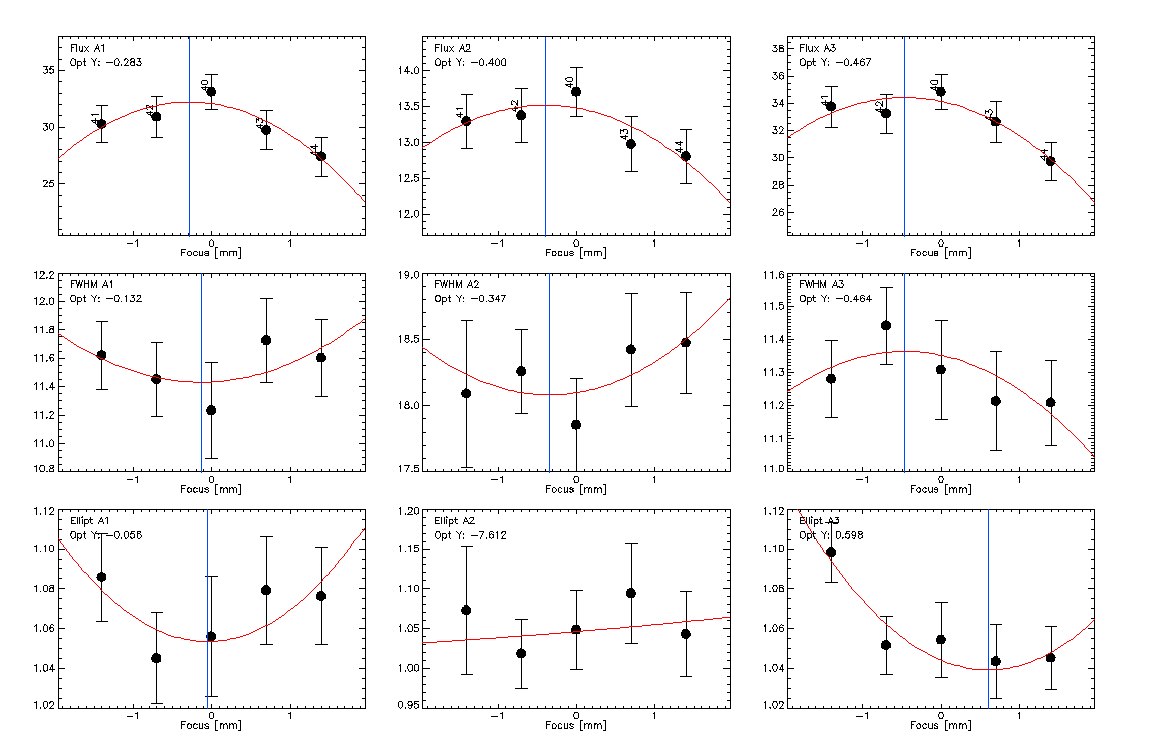
\includegraphics[height=8cm]{Figures/plot_20170223s44.png}
%\hspace{0.5cm}
%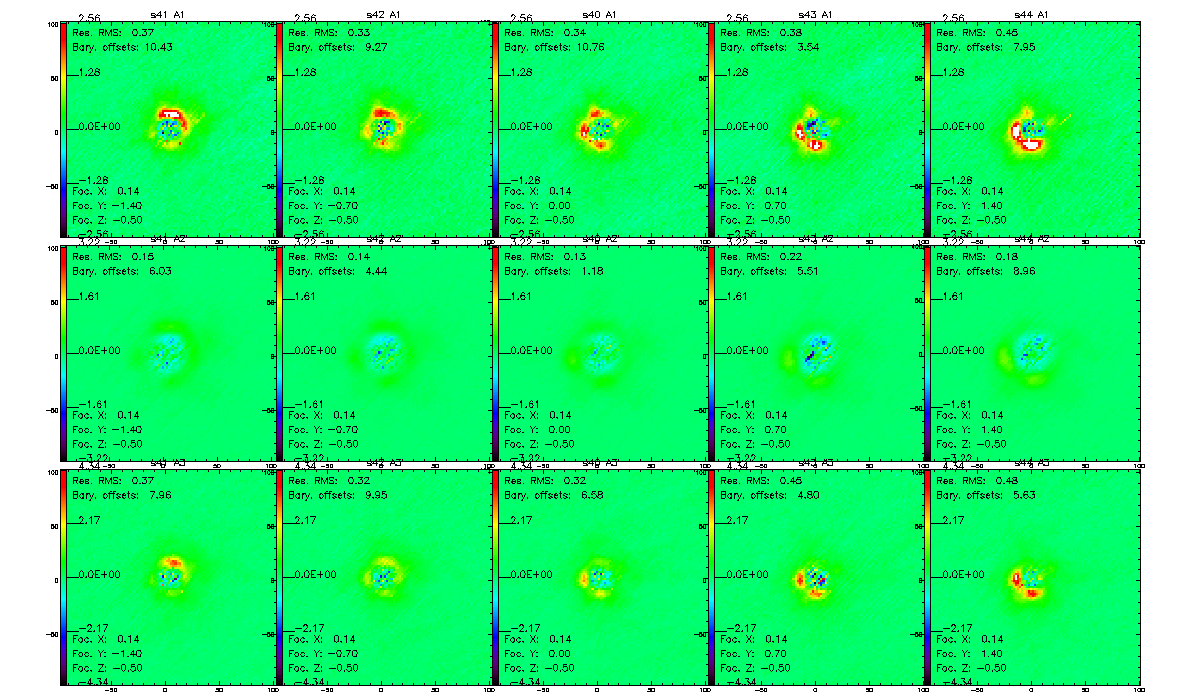
\includegraphics[height=8cm]{Figures/residuals_focus_otf_20170223s44.png}
%\caption[Lateral Y focus measures]{\emph{top panel: }Y-focus measurement using a
%    parabolic fit of the flux, beam FWHM and ellipticity on a sequence
%    of OTF scans on Uranus (20170223s44-48). \emph{bottom panel: }Beam residuals
%    after subtracting a model of the main beam for each OTF-scan of the Y-focus
%    session. (N2R9)}
%\label{fig:Y_focus}
%\end{figure*}


\subsection{Pointing}
\label{se:pointing}
% + RTA pointing estimate method
% + pointing model
% + pointing error (scan-to-scan scattering)

Once the instrument is correctly focused, we can estimate pointing corrections
before scientific observations.
%Even though EMIR only has a single pixel on the sky, the pointing procedure
%used for NIKA2 is very similar and is described in the next subsections.
%
%\paragraph{Pointing monitoring}
%
%\begin{figure}[ht!]
%\begin{center}
%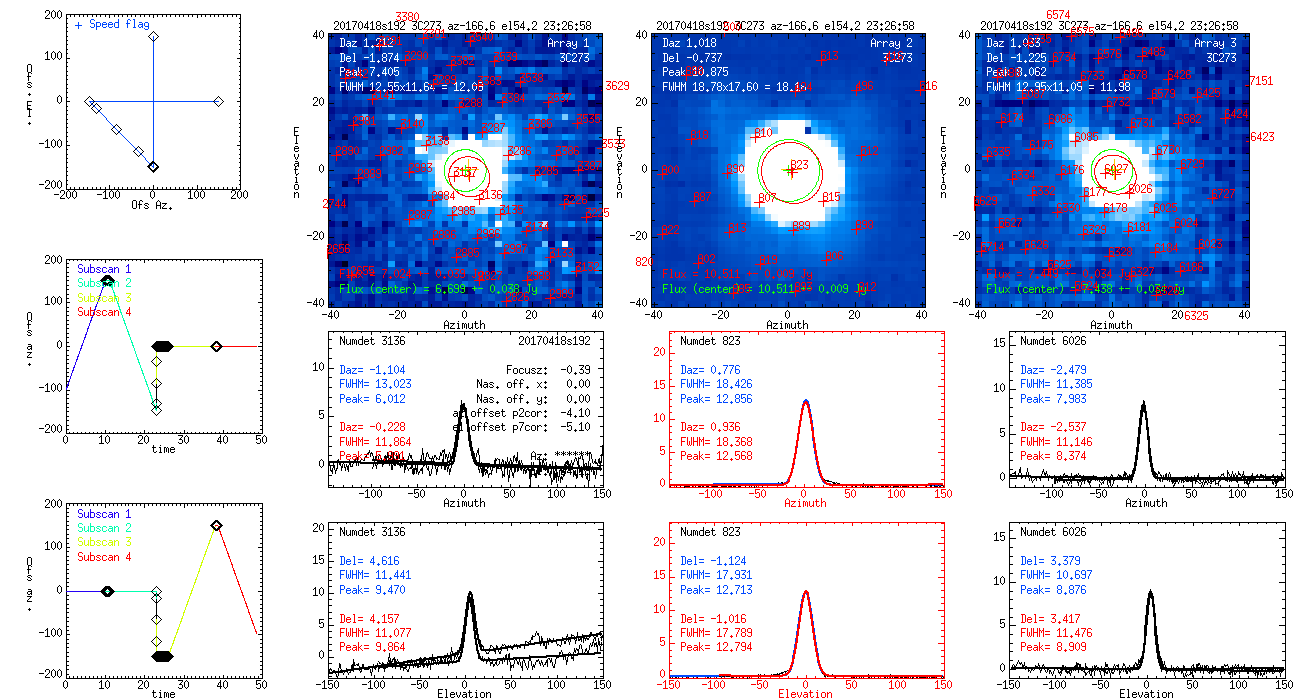
\includegraphics[clip, angle=0, scale = 0.30]{Figures/plot_20170418s192.png}
%\caption[Summary plots of the reduction of pointing scan.]{Top plots
%  show the combined map for array 1, 2 and 3, which enable a check of
%  the overall quality of the scan, while bottom plots show the set of azimuth
%  and elevation profiles for one reference detector per array. The
%  reference detector per array is highlighed with a red cross in the
%  centre of the map. The pointing reference detector of
%  \nika\ is the 2\,mm reference detector, the azimuth
%  and elevation profiles of which are shown in the central bottom
%  plot. The location of the peak in azimuth and elevation, as observed by the
%  reference detector gives the pointing offsets of the current scan.
%}
%\label{fig:ptg}
%\end{center}
%\end{figure}
%
%\begin{figure}[ht!]
%\begin{center}
%\includegraphics[clip, angle=0, trim={0, 0, 3cm, 0}, width=0.65\textwidth]{Figures/pointing_stats_N2R9.eps}
%\caption[Pointing session results]{Pointing offsets during Run9 observations,
%  before (blue to green) and after (yellow to red) the
%  derivation of Nasmyth offsets with a pointing session on Feb.~26th, 2017.}
%\label{fig:pointing_stats_n2r9}
%\end{center}
%\end{figure}
%
Based on general operating experience at the \trentemetre\ telescope, we use the so-called
{\tt pointing} or {\tt cross-type} scans to monitor the pointing during observations. The
telescope executes a back and forth scan in azimuth and a back and forth scan in
elevation, centered on the observed source. We fit Gaussian profiles
from the timelines of the reference detector, which is chosen as a
valid detector located close to the center of Array 2. We use the
estimated position of the reference detector to derive the current pointing
offsets of the system in azimuth and elevation. This correction is
propagated to the following scans. The pointing is monitored in an
hourly basis.

{\lp In addition, we perform \emph{pointing sessions} in order to
refine NIKA2 pointing model. A pointing session consists in observing
about 30 sources on a wide range of elevations and azimuth angles while
monitoring the pointing offsets that are measured for each
observation. During N2R9 technical campaign, the rms of
the residual scatter after pointing offset correction was $1.62''$ in
azimuth and $1.37''$ in elevation. We conservatively report rms pointing errors $<3''$.}
%These offsets can then
%be used to make the optical axis of the telescope to coincide with the
%optical axis of NIKA2 and thus optimize the pointing of the following scan.
%These offsets can then be passed
%to PAKO to make the optical axis of the telescope
%to coincide with the optical axis of NIKA2 and thus recenter the next scan.

%\paragraph{Pointing session}
%\label{se:pointing_session}

%Such scans and their analyses are also used to improve the pointing model of
%\nika. A pointing session consists in observing about 30 sources on a wide range
%of elevations \new{and azimuth angles} while monitoring the pointing offsets
%that are measured for each observation. These offsets are then passed to the
%IRAM staff who finds the pointing model parameters that minimize and symmetrize
%the scattering of these offsets. Based on these results, the Nasmyth offsets
%parameters that enter the IRAM pointing model are
%adjusted. Fig.~\ref{fig:pointing_stats_n2r9} shows the pointing corrections that
%had to be applied during Run9, before and after the modification of the Nasmyth
%offsets. The dispersion of the offsets is the figure of merit of the pointing
%corrections. Their distribution after the corrections (in yellow to red) is
%clearly more symmetric and narrower than before. During N2R9 run, the rms of
%the residual scatter after the correction was 1.62\,arcsec rms in
%azimuth and 1.37\,arcsec rms in elevation.


\subsection{Skydip}
\label{se:skydip}

A skydip scan consists in a step-by-step sky scan along a large range
of elevations.
{\lp NIKA2 skydips are not used for the scan-to-scan atmospheric 
calibration. For this purpose, the KIDs are used as total power
detectors to estimate the emission of the atmosphere and hence, the
atmospheric opacity, as discussed in Sect.~\ref{se:opacity}. 
NIKA2 skydips therefore serve to calibrate the KID responses with
respect to the atmospheric background for atmospheric opacity
derivation.}

Whereas with the heterodyne receivers, skydips can be
conducted continuously slewing the telescope in elevation, this
option is not feasible with NIKA2, as the KIDs need to be retuned
for a given airmass. A NIKA2 skydip, which is quoted {\tt skydip},
comprizes eleven steps in the elevation range from 19 to 65 degrees,
regularly spaced in airmass. For each step, we acquire about twenty
seconds of data to ensure a precise measurements. KIDs are tuned at
the beginning of each constant elevation sub-scan (hence once per
airmass).

{\tt Skydips} {\lp are performed once every eight hours for a wide spanning
of the atmospheric conditions thorough an observation campaign.} 


%The variation of their resonance
%frequency reads
%
%\begin{equation}
%  f_{\rm{reso}}^k  = C_0^k - C_1^k T_{atm}[1-e^{-\tau/\sin\delta}]
%\label{eq:skydip_1}
%\end{equation}

%An illustration is presented on Fig.~\ref{fig:ftone_vs_elev}. More details on
%the analysis of these {\tt skydip} scans are given in Sect.~\ref{se:opacities}.

%\begin{figure}[ht!]
%\begin{center}
%  \includegraphics[clip, angle=0, scale=0.75]{Figures/skydip_report.eps}
%\caption[skydip]{Variation of the resonance frequency of a KID
%  \new{$f_{\rm{reso}} = \ftone + \delta \ftone$},  as a function of the
%  elevation during a {\tt skydip} scan.}
%\label{fig:ftone_vs_elev}
%\end{center}
%\end{figure}

\subsection{Beam map}
\label{se:beammaps}

A \bm\ scan is a raster scan in (az,el) coordinates tailored to map a
bright compact source, often a planet, with steps of 4.8'', that are
small enough to meet Nyquist sampling of the 1\,mm beam. A scan of 
$13\times7.8$~arcmin$^2$ is acquired either with the telescope
performing a series of continuous slews at fixed elevation or at fixed azimuth. 
A continuous scanning slew defines a subscan. 
The fixed-elevation scanning has the advantage of nulling the air mass variation
across a subscan, while the fixed-azimuth scanning offers an
orthogonal scan direction to the former:
the combination of both gives a more accurate determination of the far side
lobes.
%The scan size ensures that the entire FOV is observed with good margins
%for beam mapping even on the edges and good margins for baseline derivation and
%subtraction in the scanning direction.
The scan size is optimized to enable maps to be made for all
KIDs, even those located at the edges of the array. Larger size in the scanning
direction allows for correlated noise subtraction.
During subscans, the telescope moves at
65\,arcsec/s. This value results of a tradeoff between the need to scan as
fast as possible to minimize atmospheric contamination and the
necessity to keep subscans no shorter than 10\,s (telescope antenna 
constraint). The need to have Nyquist sampling of 11'' beams along the
scan direction translates into a maximum speed of 97\,arcsec/s
for our nominal acquisition rate of 23.8\,Hz and is thus met with margins. Subscans
last 12\,s, the entire scan lasts about 25\,min.%, which is short enough
%to minimize the contribution of the atmospheric fluctuations. 
% Alessandro advice: cancel the following part of the sentence: not true in absolute
% (depending on the atmospheric conditions)
%, which is short enough to prevent
%losing the signal due to atmosphere-induced (1/f) background variations that would
%move the resonance away from the tone probing it.

{\tt Beammaps} are key observations for the calibration. {\lp Whereas
a single \bm\ acquired in stable observing conditions could suffice,
\bm\ scans are performed on a daily basis.}
More details on these observations are given in Sect.~\ref{se:geometry}
where we describe how to actually exploit them to derive individual KID
properties.

